\documentclass{article}


\include{stddefs}
\include{imodefs}

\begin{document}


\chapterno{6}
\chapter{Convex functions}\label{chapter:convexfunctions}

In this chapter we will dive deeper into convex functions. 
The main focus will be convex functions defined on intervals (convex subsets) of the
real numbers i.e. convex functions in just one variable. Along the way, differentiability is
introduced along with several classical results. We will sketch surrounding ideas, but skip 
proofs of some of the main results.

In this chapter $\log(x)$ denotes the logarithm with base $e$.


\section{Strictly convex functions}

Below we strengthen Definition \ref{Def:convexfunction} of a convex function.

\begin{definition}[emph]
  Let $C \subseteq \RR^d$ be a convex subset.
    A \emph{strictly convex function} is a convex function $f: C\rightarrow \RR$, such that
    $$
    f((1 - t) x + t y) < (1-t) f(x) + t f(y)
    $$
    for every number $t$ with $0< t < 1$ and $x\neq y$. 
  \end{definition}

\begin{frameit}  
  \begin{figure}\label{fignonstrict}
    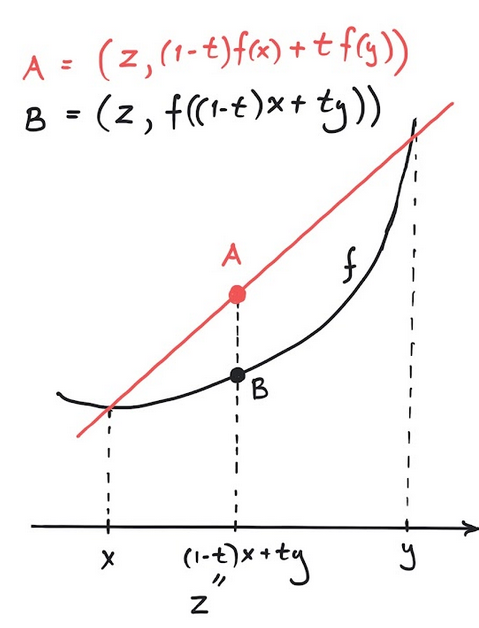
\includegraphics{strconvex.png}
    
Strictly convex function. The line segment between $(x, f(x))$ and $(y, f(y))$ lies \emph{strictly} ($<$) above
the graph of  $f$.
  \end{figure}
  \end{frameit}


  \begin{example}
    Consider the line (function) $f:\RR\rightarrow \RR$ given by
    $$
    f(x) = a x + b
    $$
    for $a, b\in \RR$.
    This function is convex, since we can formally write for every $t\in \RR$:
    \begin{align}\label{notstrconv}
      f((1-t) x + t y) &= a ((1-t) x + t y) + b \\
                       &= a ((1-t) x) + (1-t)b + a (t y) + t b\\
                       &= (1-t)(a x + b) + t(a y + b)\\
                       &= (1-t) f(x) + t f(y).
    \end{align}
    However, the computation in \eqref{notstrconv} also shows why
    there is no chance that $f(x)$ is strictly convex. Intuitively,
    the graph of convex functions need to bend and curve a bit to
    be strictly convex. No lines should occur in their graphs. 
  \end{example}

  \beginshex
  Let $f$ be a convex function. Show $f$ is strictly convex if and only if
  $$
  f((1-t) x + t y) = (1-t) f(x) + t f(y)
  $$
  for $0 < t < 1$ implies that $x=y$.
  \endshex

  \beginshex
  Give an example of a non-constant convex function $f:\RR\rightarrow \RR$, which is not strictly convex. Show in
  details that $f(x) = x^2$ is a strictly convex function.

  \begin{hideinbutton}{Hint}
    Look back to the relevant part of Exercise \ref{exconvfct} for
    dealing with $f(x) = x^2$.
    \end{hideinbutton}
  \endshex



  

\section{Why are convex functions interesting?}

  We begin this section by giving the following result without proof.

  \begin{theorem}[emph]\label{opencvxcont}
    A convex function defined on an open convex subset is continuous.
  \end{theorem}

  \beginshex
  Give an example showing that Theorem \ref{opencvxcont} is not true if the convex function
  is defined on a closed convex subset.

  \begin{hideinbutton}{Hint}
    Try to come up with an example like $f: [0, 1] \rightarrow \RR$. Look at
    the end point $0$.
    
    \begin{hideinbutton}{Hint}
      Well, try out
      $$
      f(x) =
      \begin{cases}
        1&\text{if } x = 0\\
        x&\text{if } x > 0
      \end{cases}
      $$
    \end{hideinbutton}
    \end{hideinbutton}
  \endshex

  

Let us now define precisely what is meant by a local vs a global minimum
for a function.


\begin{definition}[emph]\label{Def:localglobalmin}
Let $f: S\rightarrow \RR$ be a function, where $S\subseteq\RR^d$ is an
arbitrary subset (not necessarily convex, open or closed). Then
$x_0\in S$ is called a \emph{local minimum} for $f$ if
$$
f(x_0)\leq f(x)
$$
for every $x\in S$, which is sufficiently close to $x_0$. Being
sufficiently close to means that $x\in S$ satisfies
$$
| x - x_0 | < \epsilon
$$
for some fixed $\epsilon > 0$.

In a much stronger notion, $x_0\in S$ is called a \emph{global minimum} if
$$
f(x_0) \leq f(x)
$$
for every $x\in S$ (not just locally).
\end{definition}

\begin{frameit}
\begin{figure}
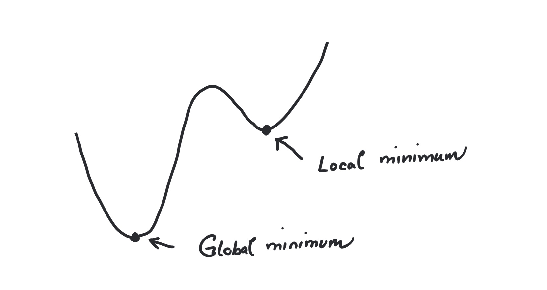
\includegraphics{localglobalmin.png}

Graph of function defined on an interval. This function has a local minimum, which is not
a global minimum.
\end{figure}
\end{frameit}


\beginshex
Give an example of a local minimum that is not a global minimum for a precisely specified function.
Also give
an example of a global minimum, which is not uniquely defined (again for a precisely specified function).
Uniquely defined means that there is precisely one $x_0$, such that $f(x_0)$ is minimal.
\endshex

We might as well have talked about maximum instead of minimum above.

\beginshex
Reformulate Definition \ref{Def:localglobalmin} in order to define
a local and a global maximum.
\endshex

A \emph{local extremum} is a point $x_0\in S$, which is either a
local minimum or a local maximum.



Convex functions $f: C\rightarrow \RR$ are interesting, because of the local
nature of the minimization problem

\begin{align}\label{cminpr}
    &\text{Minimize} &f(x)\\
    &\text{with constraint}\\
    &&x\in C
\end{align}

If you run into a local minimum in \eqref{cminpr},
then you are sure that it also is a global minimum! This is the
content of the result below. 

\begin{theorem}[emph]\label{Thm:convexoptnice}
  Let $f: C\rightarrow \RR$ be a convex function defined on a convex subset $C\subseteq \RR^d$. If $x_0\in C$ is a
  local minimum, then $x_0$ is a global minimum. If $f$ is strictly
  convex, then a global minimum for $f$ is unique.
\end{theorem}
\begin{proof}[showhide]
 By the definition of local minimum in Definition \ref{Def:localglobalmin}, there exists $\epsilon > 0$, such that $f(x_0)\leq
  f(x)$, when $x \in C$ and $\abs{ x - x_0 }< \epsilon$. Suppose that
  $x_0$ is not a global minimum. Then there exists $x_1\in C$ with
  $f(x_1) < f(x_0)$. Consider the point
  \begin{equation*}
    x_t = (1 - t) x_0 + t x_1\in C,
  \end{equation*}
  where $0 < t < 1$. Then
  \begin{equation*}
    f(x_t) \leq (1-t) f(x_0) + t f(x_1) < (1-t) f(x_0) + t f(x_0) =
    f(x_0).
  \end{equation*}
  Since $\abs{ x_t - x_0 } = t \abs{ x_1 - x_0 }$, we can choose $t >
  0$ sufficiently small such that $\abs{ x_t - x_0 } < \epsilon$
  implying $f(x_0)\leq f(x_t)$, since $x_0$ is a local minimum. This
  contradicts that $f(x_t) < f(x_0)$ for every $0 < t < 1$.  Let $f$
  be strictly convex and let $x_0$ be a global minimum for $f$. If
  $x_1\in C$, $x_1\neq x_0$ and $f(x_1) = f(x_0)$, then
  \begin{equation*}
    f((1-\lambda) x_0 + \lambda x_1) < (1-\lambda) f(x_0) + \lambda f(x_1)
    = f(x_0)
  \end{equation*}
  for $0 < \lambda < 1$. This would contradict that global minimality
  of $x_0$, since $x_0\neq (1-\lambda)x_0 + \lambda x_1\in C$ for $0<
  \lambda < 1$.
\end{proof}


The following little result turns out to be very useful and
also very intuitive and drawable! It is a key component
in characterizing convex differentiable
functions $f(x)$ in terms of $f''(x)$. We will not give the proof here.

\begin{lemma}[emph]\label{littleconvresult}
  Let $f:[a,b]\rightarrow \RR$ be a convex function. Then
  \begin{equation*}
    \frac{f(x) - f(a)}{x - a} \leq
    \frac{f(b)-f(a)}{b - a} \leq \frac{f(b)-f(x)}{b - x}
  \end{equation*}
  for $a < x < b$.
\end{lemma}

\begin{frameit}
\begin{figure}

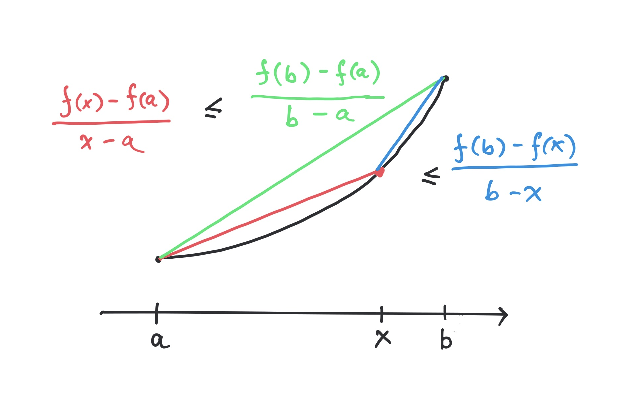
\includegraphics{geomlemmaconv.png}

The result in Lemma \ref{littleconvresult} is depicted above. A formal proof can be
given from first principles only using Definition \ref{Def:convexfunction}.
\end{figure}
\end{frameit}

\section{Differentiable functions}


To appreciate the depth of the notion of differentiability, you should
read the story (joke, actually) in the second paragraph of \url{section
  8-2}{http://www.feynmanlectures.caltech.edu/I_08.html} in volume I
of the famous \url{Feynman Lectures on Physics}{http://www.feynmanlectures.caltech.edu/}. Below is a
  photograph of the \url{master explainer}{https://en.wikipedia.org/wiki/Richard_Feynman} in action.

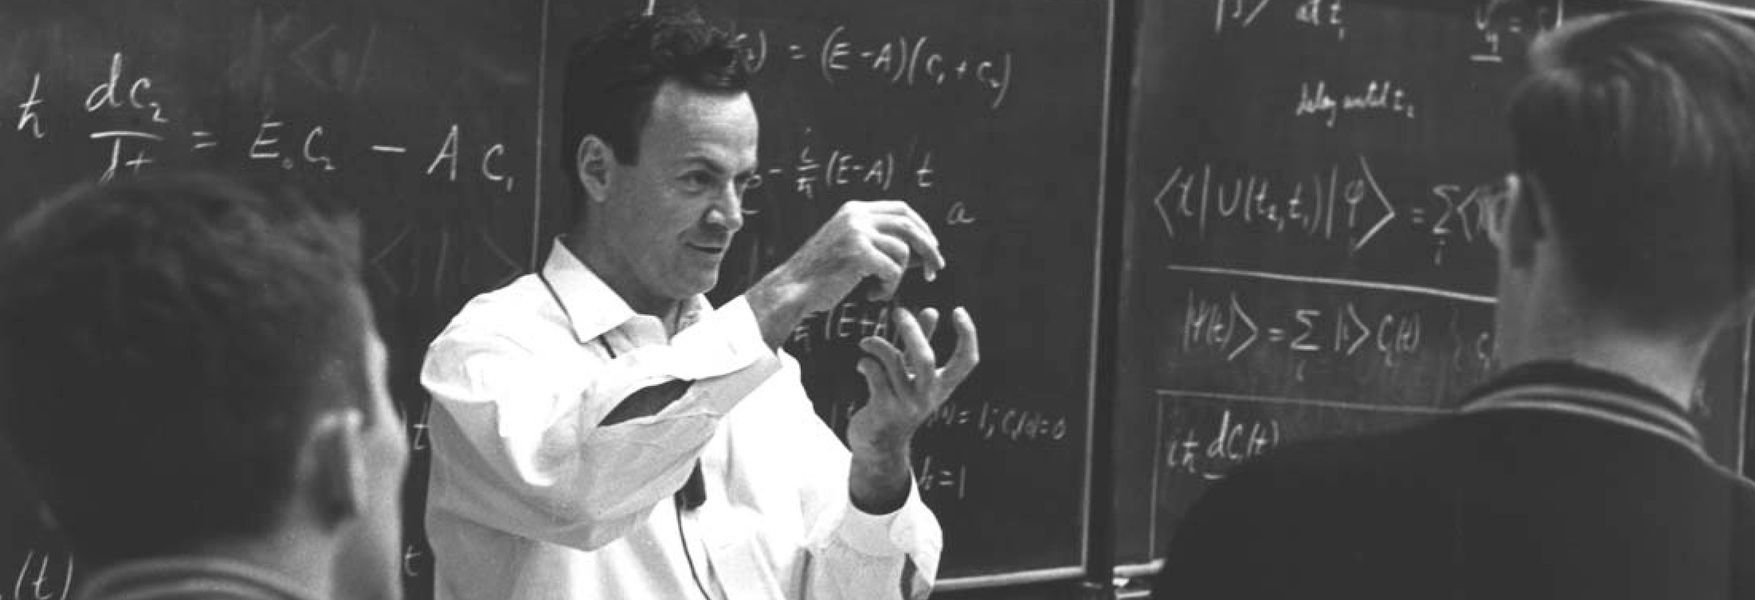
\includegraphics{Feynman.jpeg}

\subsection{Definition}

Let $f:(a, b)\rightarrow \RR$ be a function defined on the open interval $(a, b)\subset \RR$.
The notion of $f$ being differentiable at a point $x_0\in (a, b)$
can be glanced from the drawing below

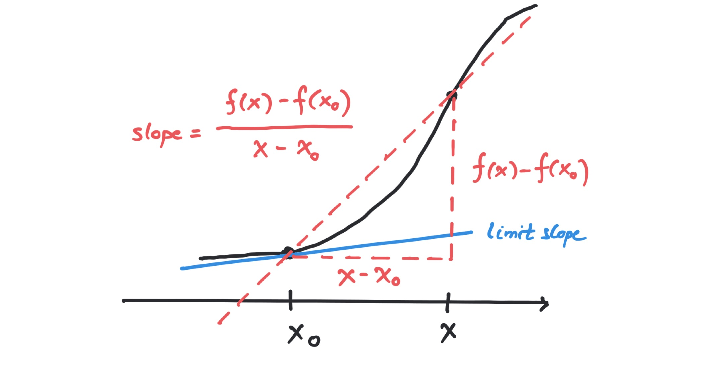
\includegraphics{limitslope.png}

where we informally let $x$ approach $x_0$ and look at the limiting
value of the slope. Newton used to say many hundred years ago, that
the derivative of $f$ at $x_0$ is the value of this slope just before
$x$ becomes $x_0$. In modern day mathematical (obfuscated?) parlance, this
gets translated into the following.

\begin{quote}
  The function $f$ is differentiable at $x_0$ if there exists a number
$c\in \RR$, such that for every $\epsilon > 0$ there exists $\delta$
with
\begin{equation}\label{defdiff0}
  \left| \frac{f(x) - f(x_0)}{x-x_0} - c \right| < \epsilon
\end{equation}
for every $x$ satisfying $|x-x_0 |<\delta$. 
\end{quote}

We will use a somewhat more operational definition below in terms
of continous functions $\epsilon$ defined around $0$ with
$\epsilon(0) = 0$. This looks difficult, but it is
actually a clever way of approaching differentiability (and more 
in the spirit of Newton).

\begin{definition}[emph]\label{defdiff}
The function $f$ is differentiable at $x_0$ if 
for some $\delta>0$, there exists a function $\epsilon: (-\delta, \delta)
\rightarrow \RR$ continuous at $0$ with $\epsilon(0) = 0$
and a number $c$, such that
\begin{equation}\label{operational}
f(x_0 + h) - f(x_0) = c h + \epsilon(h) h
\end{equation}
for $x_0 + h\in (a, b)$ and $h\in (-\delta, \delta)$. The number
$c$ is denoted $f'(x_0)$ and called \emph{the derivative} of
$f$ at $x_0$; $f$ is called \emph{differentiable} if
its derivative exists at every $x_0\in (a, b)$.
\end{definition}

\begin{remark}[emph]
  If a function $f:(a, b)\rightarrow \RR$ is
  differentiable, we get a new function
  $f':(a, b)\rightarrow \RR$ giving the (first) derivative at
  a point as output. We may ask again if this function
  is differentiable. If this is so, we may define a
  function $f'':(a, b)\rightarrow \RR$ given by
  $f''(x) = (f')'(x)$ called the second derivative. This
  procedure may be continued. We use the notation
  $f^{(n)}$ for the $n$-th derivative.
\end{remark}

\begin{example}
Let us apply Definition \ref{defdiff} to the function $f(x) = x^2$ at
the point $x_0$. Here
$$
(x_0 + h)^2 - x_0^2 = 2 x_0 h + h^2.
$$
Here you immediately see that $f'(x_0) = 2 x_0$ with
$\epsilon(h) = h$.
\end{example}

\beginshex
Use Definition \ref{defdiff} to formally show that $f'(x) = 3 x^2$
if $f(x) = x^3$.
\endshex

\begin{remark}[emph]

In operating with differentiable functions you are supposed to draw on
your previous knowledge. I have summarized some of this knowledge below (even though we will give hints below as how to prove some of the rules).


  \begin{enumerate}
\item
  If $f(x) = a g(x)$, where $a\in \RR$, then
  $$f'(x) = a g'(x)$$.
\item
If $f(x) = x^n$, where $n \in \NN$, then $$f'(x) = n x^{n-1}.$$
\item 
If $f(x) = e^x$, then  $$f'(x) = f(x) = e^x.$$
\item
If $f(x) = \log(x)$, then $$f'(x) = 1/x.$$
\item
If $f(x) = \sin(x)$, then $$f'(x) = \cos(x).$$
\item
If $f(x) = \cos(x)$, then $$f'(x) = -\sin(x).$$
\item
  If $f(x)$ and $g(x)$ are differentiable functions, then the derivative of their product is
  $$
  (f g)'(x) = f'(x) g(x) + f(x) g'(x).
  $$
\item
   If $f(x)$ and $g(x)$ are differentiable functions, then the derivative of their quotient is
  $$
  \left(\frac{f(x)}{g(x)}\right)' = \frac{f'(x) g(x) - f(x) g'(x)}{g(x)^2}.
  $$
\item
     If $f(x)$ and $g(x)$ are composable differentiable functions, then the derivative of their composite is
  $$
  (f\circ g)'(x) = f'(g(x)) g'(x).
  $$ 
\end{enumerate}
\end{remark}

\beginshex
Suppose that $f(x) = \sin(x)$. What is
$$
f^{(17)}(x)?
$$
\endshex


\subsection{Recall the derivative of a product?}

From high school you know that the derivative of a product of two functions $f$ and $g$
is given by the formula

\begin{equation}\label{hsproduct}
(f g)'(x) = f'(x) g(x) + f(x) g'(x).
\end{equation}

We can use the $\epsilon$-definition \eqref{operational} to derive the product rule
in \eqref{hsproduct}. The computation below is a bit cumbersome, but actually quite
doable. We assume to begin with that $f$ and $g$ are differentiable at $x_0$
according to \eqref{operational} i.e.,

\begin{align*}
  f(x_0 + h) &= f(x_0) + f'(x_0)h + \epsilon_f(h) h\\
  g(x_0 + h) &= g(x_0) + g'(x_0)h + \epsilon_g(h) h.\\
\end{align*}
Then we start the computation:
\begin{align}\label{prrulecomp}
&(f g)(x_0 + h) = f(x_0 + h) g(x_0 + h) =\\
  &(f(x_0) + f'(x_0)h + \epsilon_f(h) h)\,\, (g(x_0) + g'(x_0) h + \epsilon_g(h) h) =\\
  &f(x_0) g(x_0) + (f'(x_0) g(x_0)  + f(x_0) g'(x_0)) h + \epsilon(h) h,
\end{align}
where the function
\begin{equation}\label{bigcompdiffproduct}
\epsilon(h) = f(x_0) \epsilon_g(h) + f'(x_0) g'(x_0) h + f'(x_0) \epsilon_g(h) h + \epsilon_f(h) g'(x_0) +
\epsilon_f(h) g'(x_0) h + \epsilon_f(h) \epsilon_g(h) h
\end{equation}
is seen to be continuous at $h=0$ with $\epsilon(0) = 0$.
The end result of this computation shows that $f g$ is differentiable at $x_0$ with
\begin{equation}\label{prrule}
(f g)'(x_0) = f'(x_0) g(x_0) + f(x_0) g'(x_0)
\end{equation}
again according to \eqref{operational}.

\beginshex
Show that the $\epsilon$ function defined in \eqref{bigcompdiffproduct} satisfies the
relevant conditions in Definition \ref{defdiff}.
\endshex

The formula for the derivative of a fraction i.e.,
$$
\left(\frac{f(x)}{g(x)}\right)' = \frac{f'(x) g(x) - f(x) g'(x)}{g(x)^2}
$$
can be derived using a neat little trick. This is the topic of the following exercise.

\beginshex
Show how the product rule may be used to derive the rule for finding the derivative of
a fraction:
$$
\left(\frac{f}{g}\right)'(x_0) = \dfrac{f'(x_0) g(x_0) - f(x_0) g'(x_0)}{g(x_0)^2}.
$$

\begin{hideinbutton}{Hint}
  $$
  f'(x) = \left(g(x) \left(\frac{f(x)}{g(x)}\right)\right)'.
  $$
  \end{hideinbutton}
\endshex
\subsection{Recall the one variable chain rule?}

The formula for the derivative of a composite function is given by
$$
(f\circ g)'(x_0) = f'(g(x_0)) g'(x_0),
$$
where $g(x_0)$ is in the domain of $f$. Let us see how \eqref{operational}
applies in showing this.

Suppose that $f$ is differentiable at $g(x_0)$ and $g$ is
differentiable at $x_0$, then we can mess around a bit
with the $\epsilon$-functions for $f$ and $g$ for
the composite function $f(g(x))$ around $x_0$:
\begin{align*}
f(g(x_0 + h)) &= f(g(x_0) + g'(x_0) h + h \epsilon_g(h))\\
  &= f(g(x_0)) + f'(g(x_0)) g'(x_0) h + \epsilon(h) h,
\end{align*}
where (take a deep breath)
$$
\epsilon(h) = f'(g(x_0)) \epsilon_g(h) + \epsilon_f(g'(x_0) h + \epsilon_g(h)h) g'(x_0).
$$
Here $\epsilon$ is seen to be continuous at $0$ with $\epsilon(0)=0$ i.e.,
the composition $f(g(x))$ is differentiable at $x_0$ with
derivative
\begin{equation}\label{formulacompdiff}
(f\circ g)'(x_0) = f'(g(x_0)) g'(x_0).
\end{equation}

The formula \eqref{formulacompdiff} is extremely important and useful. We give some applications in
the exercises below.

\beginshex
Compute the derivative of the function $f: (0, \pi) \rightarrow \RR$ given by
$$
f(x) = \dfrac{1}{\sqrt{\sin(x)}}
$$
using only paper and pencil! You can check your result afterwards using a computer.
\endshex

\beginshex
Suppose that $g$ and $f$ are inverse functions i.e.,
$$
f(g(x)) = x\qquad \text{and} \qquad g( f(x)) = x.
$$
If you know the derivative of $f$, how can you use the chain rule
to get the derivative of $g$? Illustrate with examples like
$f(x) = x^2$ and $g(x) = \sqrt{x}$, $f(x) = e^x$ and $g(x) = \log(x)$.
\endshex


\beginshex
Suppose that $f:\RR\rightarrow \RR$ is a convex function. We know that
$f$ is continuous, but is $f$ differentiable at every point $x_0\in \RR$?

\begin{hideinbutton}{Hint}
  Nope. This is wrong. Come up with a convex function $f$ and a point $x_0$,
  such that $f$ is not differentiable at $x_0$.
\end{hideinbutton}
\endshex

\subsection{The Newton-Raphson method for finding roots}

We begin this section with a surprising example.



\begin{example}
Suppose that $a> 0$ and we wish to compute $\sqrt{a}$. To do this we may focus on the
quadratic equation $f(x) = x^2 - a = 0$ and attempt to compute an approximate value $x_0\geq 0$,
such that $f(x_0)$ is close to $0$. Let me at this point disclose that there is
a very effective iterative scheme for doing this. You start by putting $x_0 = a$ and then iterate
using the formula
\begin{equation}\label{sqnewton}
x_{i+1} = \frac{1}{2}\left(x_i + \frac{a}{x_i}\right)
\end{equation}
to get better and better approximations $x_0, x_1, x_2, \dots$ to $\sqrt{a}$. 

\begin{openeyes}
The formula in \eqref{sqnewton} is derived from 
$$
x_{i+1} = x_i - \frac{f(x_i)}{f'(x_i)},
$$
where $f(x) = x^2 - a$.
\end{openeyes}


You can try out \eqref{sqnewton}
below.

\begin{sage}
a = 2.0 
# Note a = 2.0 instead of a = 2. We need Sage to output decimal numbers - not fractions.
numberOfIter = 10 

def onestep(x):
  return (x + a/x)/2

z = a
for i in range(numberOfIter):
  z = onestep(z)
  print(z)
\end{sage}
\end{example}

I have been in complete awe of the \url{Newton-Raphson method}{https://en.wikipedia.org/wiki/Newton\%27s_method} since my early youth. It is
an algorithm, where the notion of differentiability really shines.

The method
comes from Definition \ref{defdiff} with $h = x - x_0$:
we are assuming that $x_0$ is very close to $x$, where $f(x) = 0$. Then
$$
f(x) - f(x_0) = f'(x_0) (x- x_0) + \text{a very small number}.
$$
Ignoring the very small number and solving this equation for $x$ we get
$$
x = x_0 - \frac{f(x_0)}{f'(x_0)}.
$$

In the Sage window below, I have entered the algorithm starting
in $x_0 = 0$ running ten iterations for finding a zero for
$f(x) = \cos(x) - x$.

\begin{hideinbutton}{Graph}
  \begin{sage}
    plot(cos(x) - x, (x, 0, 2*pi))
  \end{sage}
\end{hideinbutton}

\begin{sage}
x = var('x')
f(x) = cos(x) - x
df = diff(f, x)
NR(x) = x - f(x)/df(x)

x0 = 0 # initial value
n = 10 # number of iterations

for i in range(n):
  print( x0)
  x0 = N(NR(x0), digits = 10)
\end{sage}



\beginshex
Give an example, where the Newton-Raphson method cycles between points
and never finds the desired zero. Perhaps a drawing will help here.
\endshex

The Newton-Raphson converges rapidly in most cases. Of course, it
breaks down violently if it runs into a \emph{critical point} i.e.,
a point $x$, such that $f'(x) = 0$.

William Cook has made some nice Sage code available for
\url{experimentation}{https://billcookmath.com/sage/calculus/Newtons_method.html} with Newton's method.

\begin{example}
  The formula (see button in Example \ref{examplegeomseries})
  for the (monthly) payment $Y$ on a (car) loan over $N$ payments with
  a down payment of $P$ and an interest rate of $r$ (per payment or term) is given by the formula
    $$
    Y = \frac{r P}{1 - \left(\frac{1}{1+r}\right)^N}.
    $$
    There is no explicit formula for calculating $r$ given $Y, P$ and $N$. Here
    the Newton-Raphson method is invaluable for estimating $r$ by approximating a
    zero for the function
    $$
    r(x) = Y - \frac{x P}{1 - \left(\frac{1}{1+x}\right)^N}.
    $$
\end{example}

\beginshex
Your bank promises you a loan of $1.000.000$ DKK with yearly payments
of $45.000$ DKK over $30$ years. At the same time it claims that
its interest rate is very favorable at only $1.0$\%. Here the bank is
wrong! What is the
real interest rate?
How much money do you save (compared to the original offer from the bank) if you insist that the bank offers you
the promised interest rate of $1.0$\%?
\endshex




\subsection{Critical points and extrema}

\begin{definition}[emph]
  A critical point for a differentiable function $f:(a, b)\rightarrow \RR$ is
  a point $x_0\in (a, b)$ with
  $$
  f'(x_0) = 0.
  $$
\end{definition}


The crucial result here is the following. It seems to date back to Fermat (see \url{Fermat's theorem}{https://en.wikipedia.org/wiki/Fermat\%27s_theorem_(stationary_points)}).

\begin{lemma}[emph]\label{lemmacritone}
  Let $f : (a, b)\rightarrow \RR$ be a differentiable function. If
  $x_0$ is a local extremum for $f$, then $x_0$ is critical point i.e., $f'(x_0) = 0$.
\end{lemma}
\begin{proof}[showhide]
 Suppose that $\xi$ is a local maximum and that
  \begin{equation*}
    f(\xi + h) - f(\xi) = f'(\xi) h + \epsilon(h) h
  \end{equation*}
  according to \eqref{operational}. If $f'(\xi)>0$, then we can choose
  $\delta >0$ sufficiently small, such that $\abs{ \epsilon(h) } <
  f'(x_0)$ if $0\leq h < \delta$, since $\epsilon(0) = 0$ and
  $\epsilon $ is continuous in $0$. Therefore
  \begin{equation*}
    f(\xi +  h) - f(\xi) = (f'(\xi) + \epsilon(h)) h > 0,
  \end{equation*} 
  contradicting that $\xi$ is a local maximum.  The proof is similar
  for $f'(\xi) < 0$ and if $\xi$ is a local minimum.
\end{proof}

\beginshex
Is the converse of the above lemma true i.e., if $f'(x_0) = 0$ is
$x_0$ a local extremum?
\endshex

Theorem \ref{thmmeanvalue} below is called the mean value theorem. It is a consequence of Lemma \ref{lemmacritone}
and the extremely important Theorem \ref{thmcontcomp} about continuous functions
on compact subsets attaining their maxima and minima!


\begin{frameit}
\begin{theorem}\label{thmmeanvalue}
  Let $f:[a, b]\rightarrow \RR$ be continuous and differentiable
  on $(a, b)$. Then there exists $x_0\in (a, b)$ such that
  \begin{equation*}
    f'(x_0) = \frac{f(b) - f(a)}{b - a}.\label{xiaim}
  \end{equation*}
\end{theorem}
\end{frameit}

\subsection{Increasing functions}

The definition below is much simpler than the definition of differentiability.

\begin{definition}[emph]
A function $f:S\rightarrow \RR$ with $S\subseteq \RR$ is called
  \emph{increasing} if
  \begin{equation*}
    x\leq y\Rightarrow f(x) \leq f(y)
  \end{equation*}
  and \emph{strictly increasing} if \index{strictly increasing function}
  \begin{equation*}
    x< y\Rightarrow f(x) < f(y)
  \end{equation*}
  for $x, y\in S$.
\end{definition}

\beginshex
Give an example of an increasing function.
Give an example of an increasing function that is not strictly increasing.
\endshex

The following very important result is a consequence of Theorem \ref{thmmeanvalue}. You probably already know this result from your previous (danish) education (monotoniforhold!).

\begin{proposition}[emph]
  Let $f : (a, b)\rightarrow \RR$ be a differentiable function.
  Then
  $f$ is increasing if and only if $f'(x)\geq 0$ for every $x\in (a,
  b)$.  If $f'(x)> 0$ for every $x\in (a, b)$, then $f$ is strictly
  increasing.
\end{proposition}


\beginshex
Show that $f(x) = x^3$ is strictly increasing i.e., 
$$
x < y \implies x^3 < y^3.
$$
\begin{hideinbutton}{Hint}
$$
y^3 - x^3 = (y - x) (y^2 + x y + x^2),
$$
but why is $y^2 + x y + x^2$ always $> 0$ except when $x = y = 0$?
\end{hideinbutton}
\endshex


\beginshex
Suppose that $f: [a, b] \rightarrow \RR$ is a continuous function, such that
$f$ is differentiable on the open interval $(a, b)$. Is $f$ increasing
on $[a, b]$ if $f'(x)\geq 0$ for every $x\in (a, b)$?
\endshex

\beginshex
Is it possible for a strictly increasing function $f: \RR \rightarrow \RR$ to be bounded i.e., does
there exist a (positive) number $M$, such that $|f(x)| \leq M$ for every $x\in \RR$?

\begin{hideinbutton}{Hint}
  Have a look at
  $$
  f(x) = \dfrac{1}{1 + e^{-x}}.
  $$
  
\end{hideinbutton}
\endshex

\section{Taylor polynomials}\label{section:Taylor}

If $x_0$ is a critical point for $f$ we cannot conclude that $x_0$ is a local extremum. We know
that $f'(x_0)=0$ and we can get more information out of $f$ by exploring the signs of
$$
f''(x_0), f'''(x_0), \dots
$$

Suppose that 
$$
f(x) = a_0 + a_1 x + a_2 x^2 + \cdots + a_n x^n
$$
is a polynomial, then
\begin{equation}\label{taylor}
f(x) = f(0) + f'(0) x + \frac{f''(0)}{2} x^2 + \cdots + \frac{f^{(n)}(0)}{n!} x^n.
\end{equation}

For nice functions like $f(x) = e^x$ we can play this game ad infinitum. In fact in this
way we get the beautiful infinite series
$$
e^x = 1 + x + \frac{x^2}{2} + \frac{x^3}{6} + \cdots + \frac{x^n}{n!} + \cdots.
$$

If $f$ is an $n$ times differentiable function defined at $0$, we call
the polynomial in \eqref{taylor} the Taylor polynomial about the point $0$ of degree $n$ associated
with the $f$. Similarly, one may also define the Taylor polynomial of order $n$ about a point $a$ by
$$
f(a) + f'(a) (x-a) + \frac{f''(a)}{2} (x-a)^2 + \cdots + \frac{f^{(n)}(a)}{n!} (x-a)^n.
$$
Taylor polynomials can be used to approximate more complicated functions such as
$\cos(x)$ and $\sin (x)$ with a well defined error term. This is cool classical
mathematics. Unfortunately we do not have time to go deeper into
\url{Taylor's theorem}{https://en.wikipedia.org/wiki/Taylor\%27s_theorem}, which states this
in precise terms.

\beginshex
Compute the Taylor polynomial for $f(x) = \cos(x)$ up to degree $10$.
\endshex

\beginshex
Suppose you have a number $i$ that satisfies
$$
i^2 = -1.
$$
Can you make sense of the formula
$$
e^{i x} = \cos(x) + i \sin(x)
$$
using Taylor polynomials?
\endshex


In the context of optimization, the following
result becomes important. We will not give the proof, but only notice that Theorem
\ref{thmmeanvalue} also here plays an important role.

\begin{theorem}[emph]\label{derconv}
  Let $x_0$ be a critical point of an $n+1$ times differentiable
  function $f:(a, b)\rightarrow \RR$, such that $f^{(n+1)}$
  is a continuous function,
  \begin{align*}
    f''(x_0) &= 0\\
    f'''(x_0) &= 0\\
&\vdots\\
   f^{(n-1)}(x_0) &= 0
  \end{align*}
  and $f^{(n)}(x_0)\neq 0$. If $n$ is even, then $x_0$ is a local
  minimum if $f^{(n)}(x_0) > 0$ and a local maximum if
  $f^{(n)}(x_0)<0$. If $n$ is odd, then $x_0$ is not a local extremum.
\end{theorem}

\begin{example}\label{parabolalegs}
  Let us apply Theorem \ref{derconv} to the function
  $$
  f(x) = a x^2 + b x + c,
  $$
  where $a\neq 0$. Here $f'(x) = 2 a x + b$ and
  $$
  x_0 = - \frac{b}{2 a}
  $$
  is a critical point (why?). Since
  $$
  f''(x_0) = 2 a,
  $$
  we see that $x_0$ is a local minimum if $a > 0$ and a local maximum if
  $a < 0$.
\end{example}

\beginshex
Have you seen Example \ref{parabolalegs} elsewhere, perhaps in a more
geometric setting? What type of curve is the graph of $f(x)$? Here you may consult
your previous mathematical knowledge.

What is the outcome, when you apply Theorem \ref{derconv} to the
function $f(x) = x^3$ at $x_0 = 0$?
\endshex

\beginshex\label{exderconv}
Show that $x_0=0$ is a critical point of the function $f: (-\frac{1}{2}, \infty)\rightarrow \RR$
defined by
$$
f(x) = e^x + \log(1 + 2 x) - 3 x.
$$
Use Theorem \ref{derconv} in deciding if it is a local
maximum or minimum or neither.

\endshex

\section{Differentiable convex functions}


The following theorem is proved using Lemma \ref{littleconvresult} and
Theorem \ref{thmmeanvalue}. It immediately implies Corollary \ref{corfdp},
which is the result mostly used.


\begin{theorem}\label{fdp}
  Let $f:(a, b)\rightarrow \RR$ be a
  differentiable function. Then $f$ is convex if and only if $f'$ is
  increasing.  If $f'$ is strictly increasing, then $f$ is strictly
  convex.
\end{theorem}


Theorem \ref{fdp} leads to the following all important result.

\begin{corollary}[emph]\label{corfdp}
  Let $f:(a, b)\rightarrow \RR$ be a twice differentiable
  function. Then $f$ is convex if and only if $f''(x)\geq 0$ for every
  $x\in (a, b)$. If $f''(x) > 0$ for every $x\in (a, b)$, then $f$ is
  strictly convex.
\end{corollary}


\begin{frameit}
\begin{remark}
Wait! Stop! Why did I not write $f''(x) > 0$ if and only if 
$f$ is strictly convex?
\end{remark}
\end{frameit}

\beginshex
Can you deduce from Corollary \ref{corfdp} that the function
$f: \RR \rightarrow \RR$ given by $f(x) = x^4$ is a
strictly convex function?
\endshex

\beginshex
Show that $f(x) = e^x$ is a strictly convex function $f: \RR\rightarrow \RR$.

Show that $f(x) = -\log(x)$ is a strictly convex function
$f: (0, \infty) \rightarrow \RR$.
\endshex

\beginshex
Show that $f: \{x\in \RR \mid x \geq 0\}\rightarrow \RR$ given by
$$
f(x) = -\sqrt{x}
$$
is a strictly convex function.
\endshex


Another nice application of Lemma \ref{littleconvresult} (and Theorem \ref{fdp}) is the following.

\begin{theorem}\label{fp}
  Let $f:(a, b)\rightarrow \RR$ be a differentiable function. Then $f$
  is convex if and only if
  \begin{equation*}
    f(y) \geq f(x) + f'(x)(y-x)
  \end{equation*} 
  for every $x, y\in (a, b)$.
\end{theorem}


\beginshex
Suppose that $f:(a, b)\rightarrow \RR$ is a differentiable
convex function and $x_0\in (a, b)$ is a critical point for
$f$. What can you say about $x_0$ using Theorem \ref{fp}?
\endshex


\end{document}